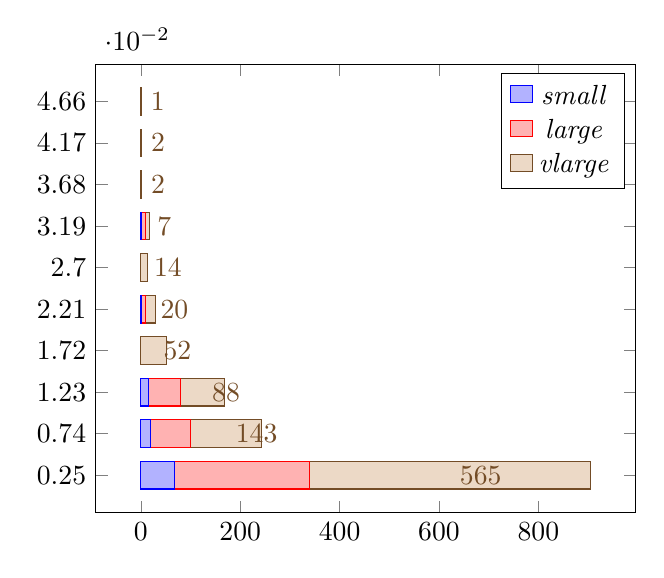
\begin{tikzpicture}
\begin{axis}[
    xbar stacked,%xbar=0pt,
%    bar width=4,
%    width=7cm,
%    height=12cm,
%    minor y tick num=4,
    ytick=data,
%    enlargelimits=0.15,
]
%\begin{axis}[xbar stacked,
%             legend style={at={(0.5,-0.20)},
%                anchor=north,legend columns=-1},
%             ylabel={Value},
%             xlabel={\#elements},
%             ]

\addplot+
coordinates{(68, 0.0025) (20, 0.0074) (16, 0.0123) (0, 0.0172) (2, 0.0221)
             (0, 0.0270) (2, 0.0319) (0, 0.0368) (0, 0.0417) (0, 0.0466)};

\addplot+
coordinates{(272, 0.0025) (80, 0.0074) (64, 0.0123) (0, 0.0172) (8, 0.0221)
             (0, 0.0270) (8, 0.0319) (0, 0.0368) (0, 0.0417) (0, 0.0466)};

\addplot+[
          nodes near coords,
          nodes near coords align={horizontal}
         ]
coordinates{(565, 0.0025) (143, 0.0074) (88, 0.0123) (52, 0.0172) (20, 0.0221)
             (14, 0.0270) (7, 0.0319) (2, 0.0368) (2, 0.0417) (1, 0.0466)};

\legend{\textit{small}, \textit{large}, \textit{vlarge}}
    
\end{axis}
\end{tikzpicture}
